\documentclass{article}
\usepackage[svgnames]{xcolor}
\usepackage[a0paper,landscape,margin=3cm]{geometry}
\usepackage[utf8]{inputenc}
\usepackage[sorting=nyt,backend=biber,style=authoryear,block=par]{biblatex}
\usepackage{anyfontsize}
\usepackage{tikz}
\usepackage{mathpazo}
\usepackage{multicol,caption}
\usepackage{tikz}
\usepackage{graphicx}
\usepackage[inkscapeformat=png]{svg}
\usepackage{blindtext}
\usepackage[inkscapeformat=png]{svg}
\usepackage{booktabs}
\usetikzlibrary{matrix,fadings,arrows,trees,calc,positioning,decorations,automata,fit,backgrounds}
\pagecolor{red!5}

\columnsep=50pt
% \columnseprule=2pt
\graphicspath{ {images/} }

\renewcommand{\section}[1]{
    \begin{center}
        \begin{tikzpicture}
            \draw node[fill=white!10, text width=0.85\linewidth, text centered, inner sep=10pt, rounded corners=5pt, draw=red!80]
            {\textbf{#1}};
        \end{tikzpicture}
   
    \end{center}

}

\renewcommand{\bibfont}{}

% {\subsection*{References }}
\addbibresource{References.bib}


\renewcommand{\subsection}[1]{
    % \begin{center}
        % \begin{tikzpicture}
        %     \draw node[fill=white!10, text width=0.97\linewidth, text centered, inner sep=10pt, rounded corners=5pt, draw=red!30]
        %     {\textbf{#1}};
        % \end{tikzpicture}
        {\textbf{#1}}
    % \end{center}

}

\newenvironment{Figure}
  {\par\medskip\noindent\minipage{\linewidth}}
  {\endminipage\par\medskip}

\begin{document}
    \fontsize{55}{65}
    \selectfont
     \begin{tikzpicture}
            
        \node[inner sep=0pt] (logo) {\includesvg{SRH_Bildung.svg}}; 
        \draw node[text width=0.87\linewidth,text centered,rounded corners=5pt,inner sep=30pt,right=100pt of logo] (title){
            {Application of Natural Language Processing in an E-commerce industry}\\[0.5cm]
            \fontsize{50}{55}
            \selectfont
            {Predicting multilevel product category} \\[1cm]  
            \fontsize{40}{50}
            \selectfont
            Shoney Arickathil, Prof. Dr. Gerd Moeckel \\[0.5cm]
            \fontsize{50}{50}
            \selectfont
            Applied Computer Science, SRH Hochschule, Heidelberg
            };
    \begin{scope}[on background layer]
        \node [fill=Red!10, fit={(logo) (title)}] {};
    \end{scope}

\end{tikzpicture}
\vspace{1cm}
\begin{multicols*}{3}

   
    \fontsize{30}{35}
    \selectfont
    \section{Introduction}
    E-commerce sales are increasing exponentially ever since the world is connected online. Convinience for searching the desired product, comparing different products before making a purchase and easy access on tips of the finger has made online shoping trending especially among the youth. A vast variety of products are sold online.

    Product taxonomy (categorization) is the logical and heirarchical arrangement of the company's product. A well defined product taxonomy enables customers to search the desired product in least number of clicks on an E-commerce website. 
    An AI of unsupervised learning model to create product taxonomy based on product features is the need of the hour. In this paper, a research on automating the process of defining the product taxonomy is conducted. 
    
 
    \section{Problem statement and objective}

    In a business to business(B2B) type of E-commerse, the product taxonomy exchange between the companies such as suppliers and manufactures and online reteiler may differ. Product taxonomy must be analyzed and fit into the existing vocabular of the product taxonomy of online retailer. An example, if a supplier name a certain product category as "Engine oil" and the category already existing at online retailer is "Motor Oil". In such case importing the category from the supplier may result in poorly defined product taxonomy. The objective is to perform feature selection of product details using scikit learn \parencite{sklearn_api}, process text based classification on each heirarchy to predict the category levels of the product.

    \begin{multicols}{2}
        \section{Tools and Technologies}
            \includesvg{PyTorch_logo_black.svg} \\
            Pytorch  \parencite{Paszke.03122019} is a machine learnning library which provides Pythonic programming style. The open-source Python ecosystem packages like NumPy, SciPy and Pandas fulfills most of the numerical analysis needs of research.  Python provides vast repositories of libraries to handle data preprocessing, statistical analysis and plotting. 

            Pytorch performs execution of dynamic tensors computation with automatic differentiation for efficient gradient based optimization. 
            \columnbreak     

        \section{Research questions}
        \begin{enumerate}
            \item How Natural Language Processing (NLP) can be applied in ecommerse industry?
            \item Which neural network architecture is suitable for text based classification model?
            \item What are the steps involved for preprocessing text to extract features from the document?
            \item  How to get better results with better shaped network? Evaluate neural network performance based on confusion matrix.
        \end{enumerate}
     
    \end{multicols}


    \section{Methodology}
    Design thinking a user-centered aprroach enabled to define the problems and its solutions while developing the model which predicts multi-level product category.
    \begin{enumerate}
        \item Inspitation: Product details imported from manufactures or suppliers were needed to be  scrutinize before making these ready for deployment and publically available for customers. 
        \item Empathize: User of a "Predicting the product category" are the E-commerse industries. Gained in depth understanding of the user needs.
        \item Ideate:  Tuitorial on character-level RNN \parencite{sean} provides a basic building block for a RNN. Modifying it to work with word or vocabulary level RNN help achieve the goal of predicting category based on product features.
        \item Prototype: Creating a prototype of predicting category based on a single feature of product before including all the features.
        \item Test: Testing the prototype and gaining the feedback from the user. 
    \end{enumerate} 

    

    \section{Network Architecture - Recurrent Neural Network}
    % \begin{Figure}
    %     \centering
    %     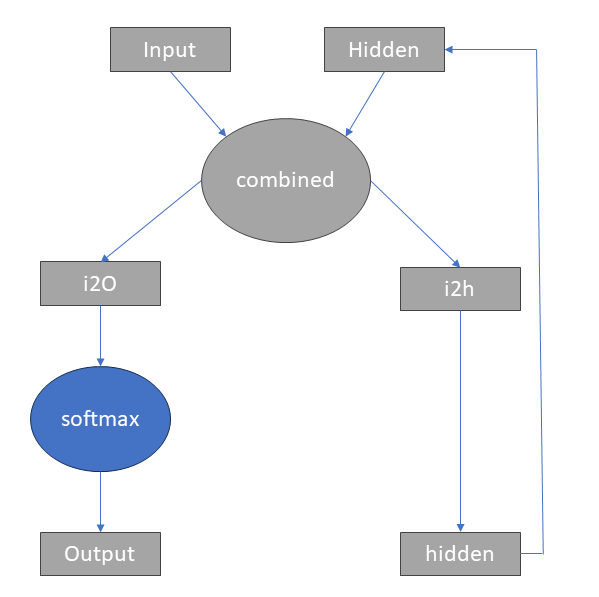
\includegraphics[width=0.50\linewidth]{nn_arch}
    %     \captionsetup{font=footnotesize}
    %     \captionof{figure}{Confusion Matrix}
    %     \label{fig:nn}
    % \end{Figure}
    

    \begin{enumerate}
        \item Input layer - These nodes pass on information to hidden nodes. The collection of product names after normalization and creating a vocabulary of it using n-gram vectorization provides provides \textit{n} number of unique words. Here, \textit{n} is the number of input layer size.  
        \item Hidden layers -  Transfers information from input node to the output node.
        \item Output layer - This layer performs computation and transfers information to the network to out of the function. In our experiment the total number of categories the model should predict is the size of the output layer.
        \item Softmax function - Takes input of \textit{K} real numbers, and normalizes it into a probability distribution consisting of \textit{K} probabilities.
        \item Combine function : Add the input layer and hidden layer tensors and pass on to the softmax function.
    \end{enumerate}



    \section{Evaluation and Results}
    \begin{enumerate}
        \item Preprocessing of the product and category data frame is performed, which involves step:-
        \begin{enumerate}
            \item Normalization of text: lowercase, perform Tf-Idf, ngram vectorization to extract text.
            \item To change \"A to A, the Normal form D (NFD) should be applied which translates each character into its decomposed form.
            \item Use Beautiful Soup a Pyhon library for pulling data out of HTLM and XML.
        \end{enumerate}
        \item The developed text based classification model successfully preditcs the product taxonomy based on the product features.
        \item The time required to analyze the product details before it is ready deploy is reduced. As manual work of defining the product taxonomy is automated.  
        \item Better shaped neural network architecture is developed. 
        
    \end{enumerate}
    \vspace{1cm}
    \subsection{Text: Before and After normalization}
    \begin{center}
        \begin{tabular}{lll}
            \toprule 
                    &\textbf{Name} & \textbf{Category} \\ 
            \midrule
            \textbf{Before}&VAICO V10-4245 Stoßdämpfer & Stoßdämpfer \\
            \textbf{After}&vaico stoßdampfer & stoßdampfer \\
        
            \bottomrule
        \end{tabular}
        
    \end{center}
\vspace{1cm}
    \subsection{Confusion Matrix}
    Confusion matrix displays how well the network performed on different categories. It is a matrix of actual categories (rows) which category the network guesses (columns). In figure \ref{fig:cm}, the yellow cells aligned diagonally shows the correct guesses by the network.

    \begin{Figure}
        \centering
        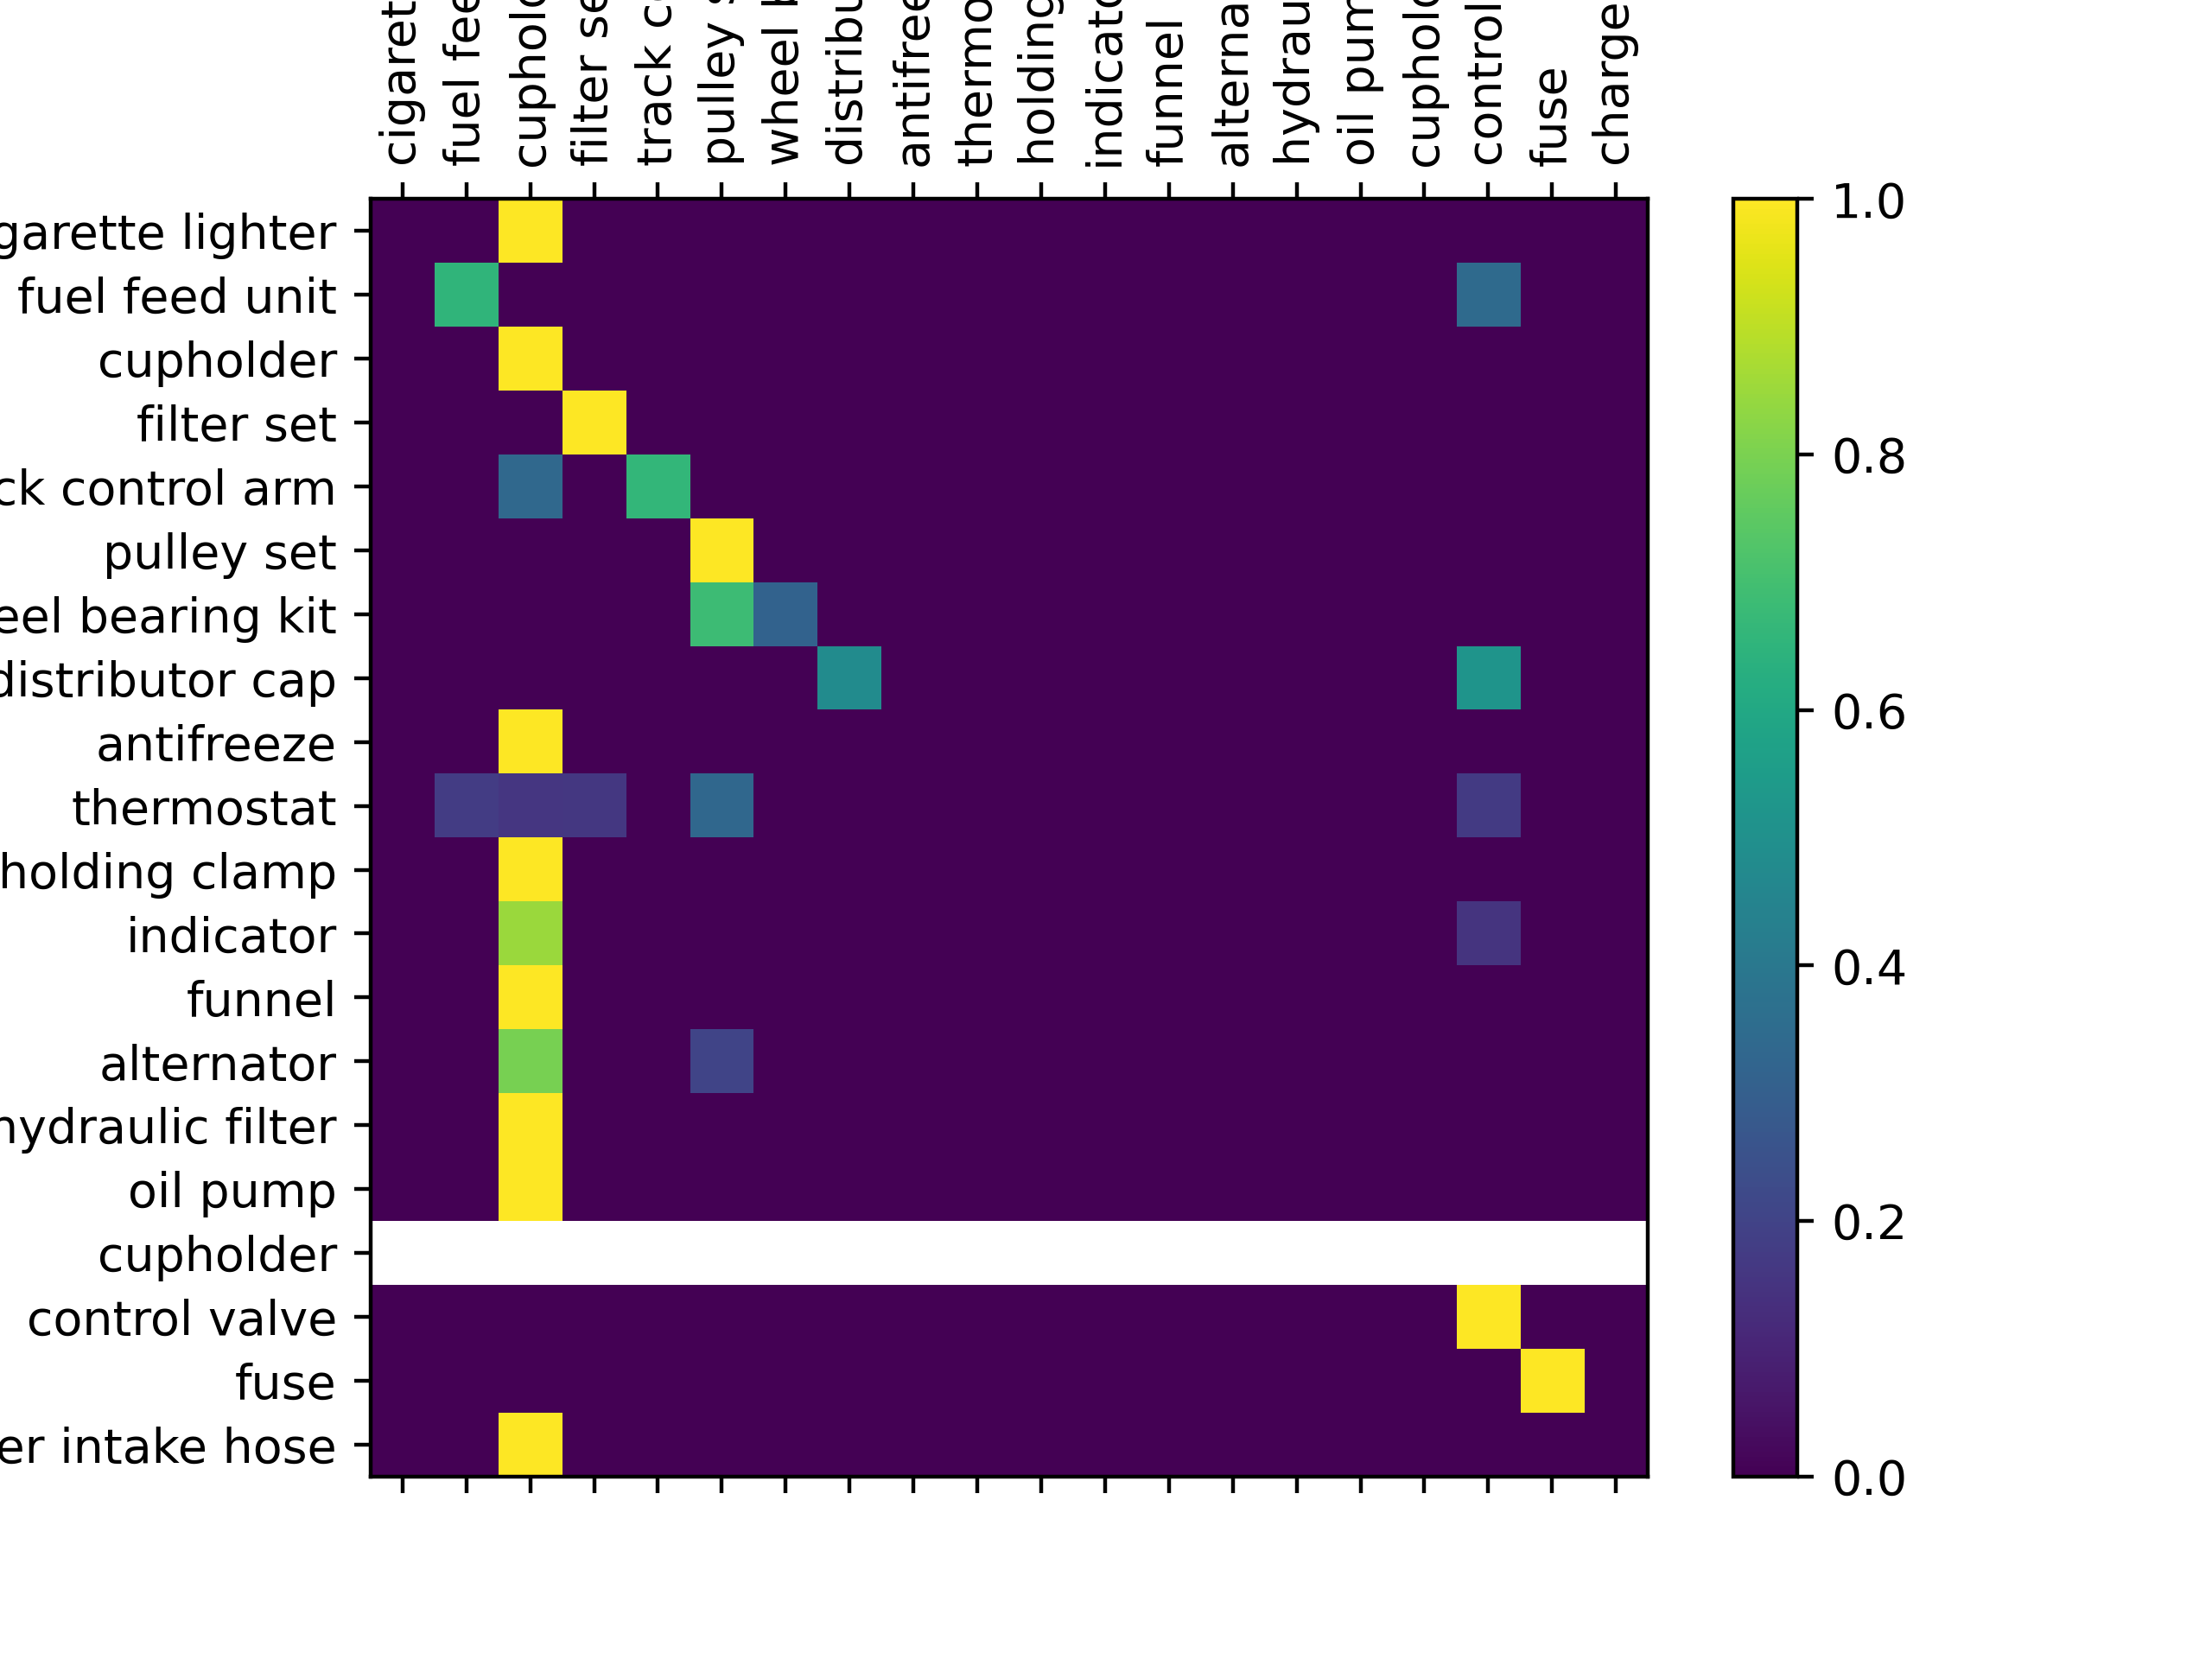
\includegraphics[width=0.50\linewidth]{confusion._200epoch}
        \captionsetup{font=footnotesize}
        \captionof{figure}{Confusion Matrix}
        \label{fig:cm}
    \end{Figure}

 \printbibliography



          
    
\end{multicols*}





\end{document}